\documentclass[../Supercritical_fluid_extraction_of_essential_oil_from_chamomile.tex]{subfiles}
\graphicspath{{\subfix{../Figures/}}}
\begin{document}
	
	\label{CH: Results}
		
	To solve the parameter estimation problem, the single shooting method was used to transform the boundary-value problem into the initial value problem and to formulate the non-linear programming problem. This non-linear optimization task was tackled using the CasADi framework (\citet{Andersson2018}). Each time series was fitted separately to the model with the linear extraction kinetics (Equation \ref{Model_kinetic_no_sat}). The initial value problem was solved multiple times with varying initial guesses to identify the global minimum. In case of the linear, two parameters remain to be determined: the partition coefficient $k_m$ and the internal diffusion coefficient $D_i$. 
	
	Figure \ref{fig: Fit_1_linear} shows the parameter space and corresponding values of the cost function for experiment 1 ($40^\circ C$, 100 bar and 6.67$\times 10^{-5}$ kg/s). As the cost function is to be minimized, the lowest value of $-\ln(L)$ indicate the best fit. A black vertical stripe at $D_i \approx 0.2$ can be observed. That stripe indicates the existence of the optimal value of the $D_i$. In the direction of $k_m$, the cost function is almost flat, which suggests that any value of $k_m$ above 0.1 fits the data equally well. If $k_m$ can be an arbitrary point, then it can grow to infinity, which suggests that the solvent is far from the saturation, and the model can be simplified. The model reduction can be introduced by considering the limit of $k_m$ in the extraction kinetic term:
	
	\begin{figure}[!h]
		\centering
		\begin{subfigure}{0.48\columnwidth}
			\centering
			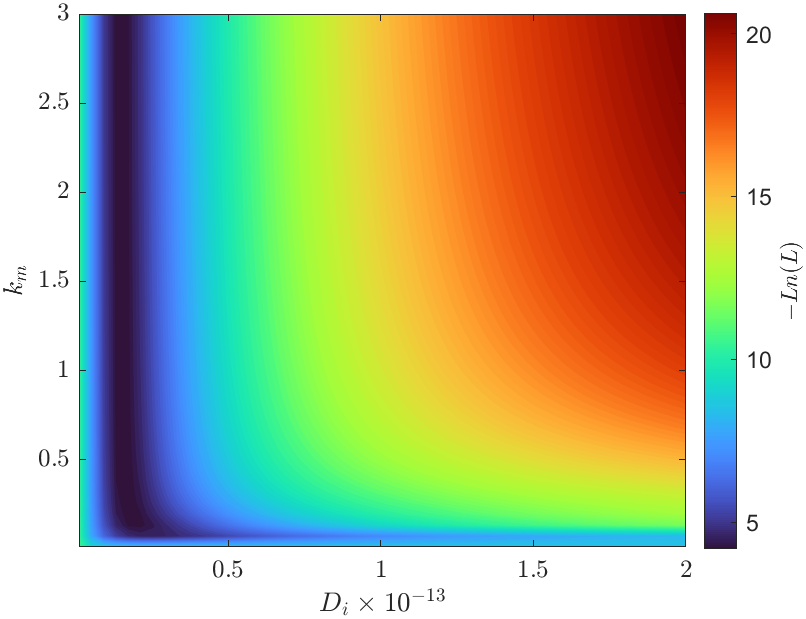
\includegraphics[trim = 0.0cm 0.0cm 0.0cm 0.0cm,clip, width=\columnwidth]{/Results_estimation/Parameter_Space_Linear_Dataset_1.png}
			\caption{The linear kinetic model \\ ~}
			\label{fig: Fit_1_linear}
		\end{subfigure}
		\hfill
		\begin{subfigure}{0.48\columnwidth}
			\centering
			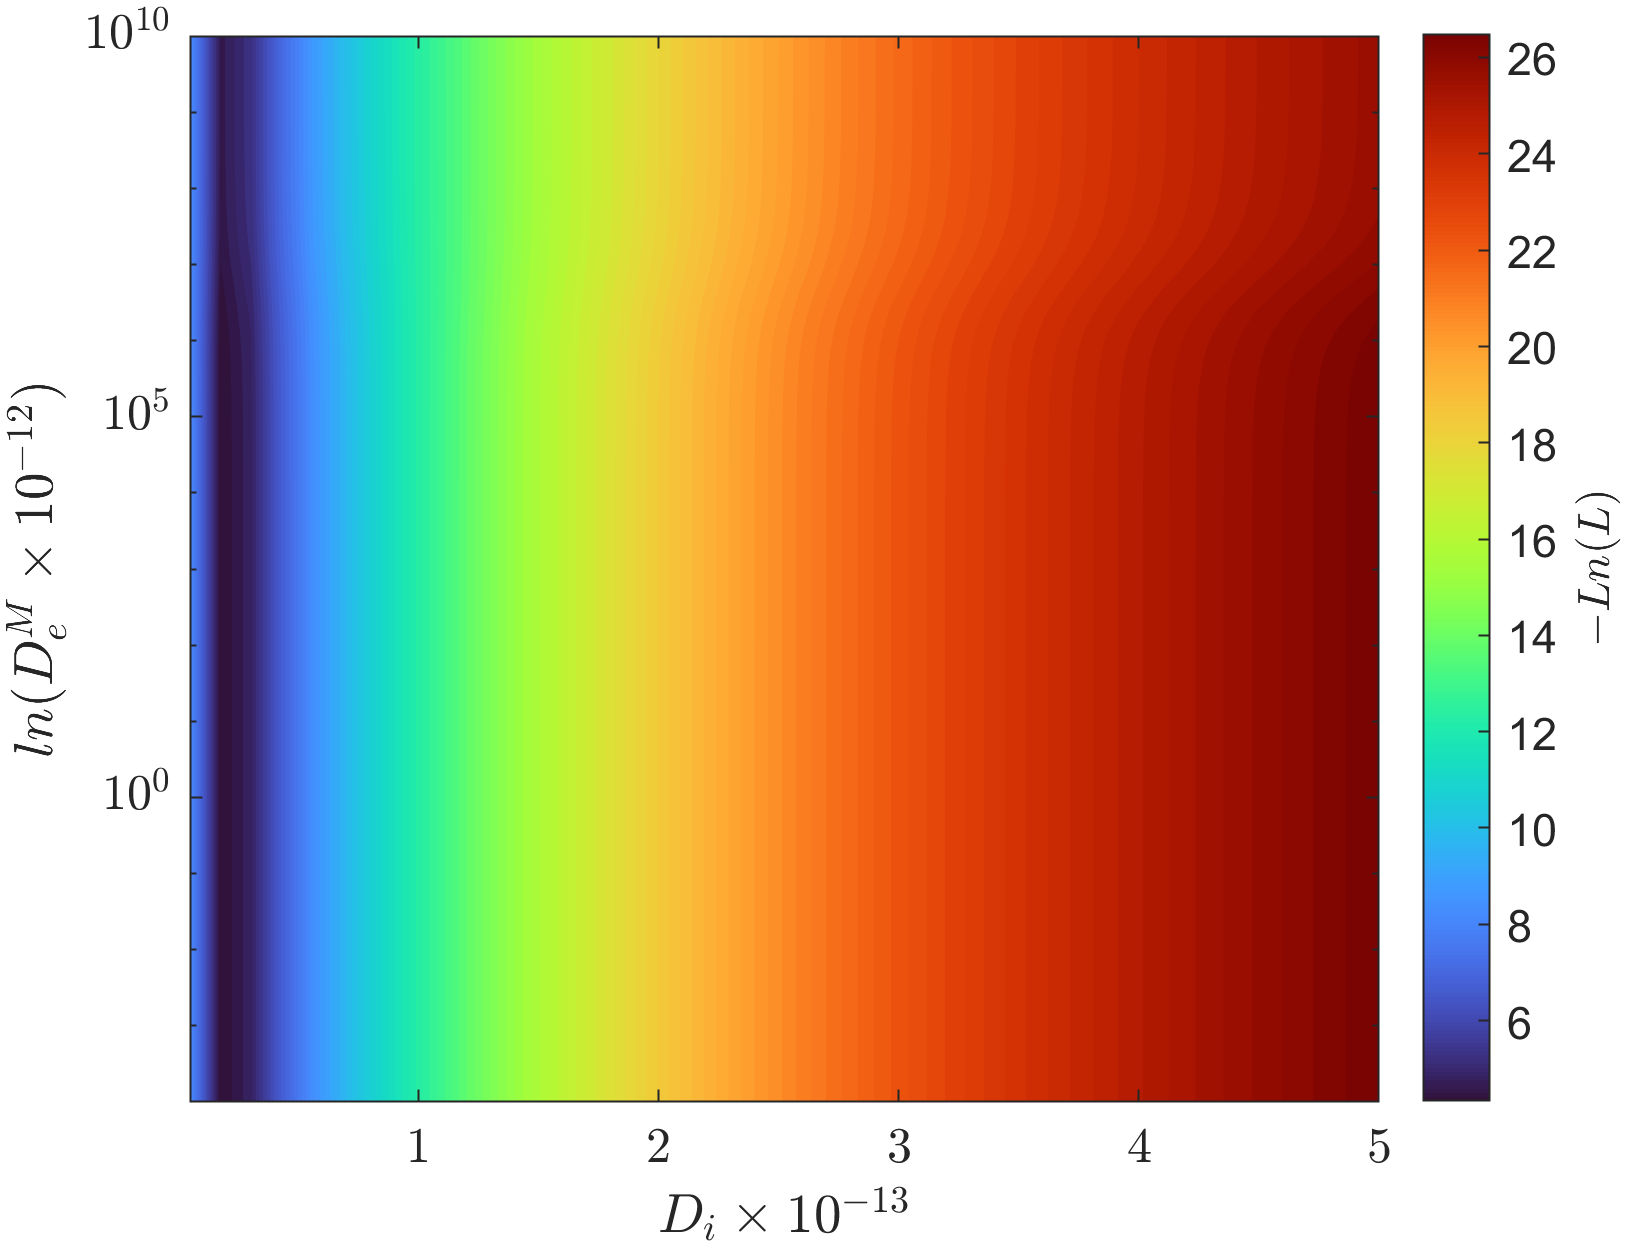
\includegraphics[trim = 0.0cm 0.0cm 0.0cm 0.0cm,clip, width=\columnwidth]{/Results_estimation/Parameter_Space_Di_Dx_Dataset_1.png}
			\caption{The reduced linear kinetic model with axial diffusion}
			\label{fig: Fit_1_Di_Dx}
		\end{subfigure}
		\hfill
		\begin{subfigure}{0.48\columnwidth}
			\centering
			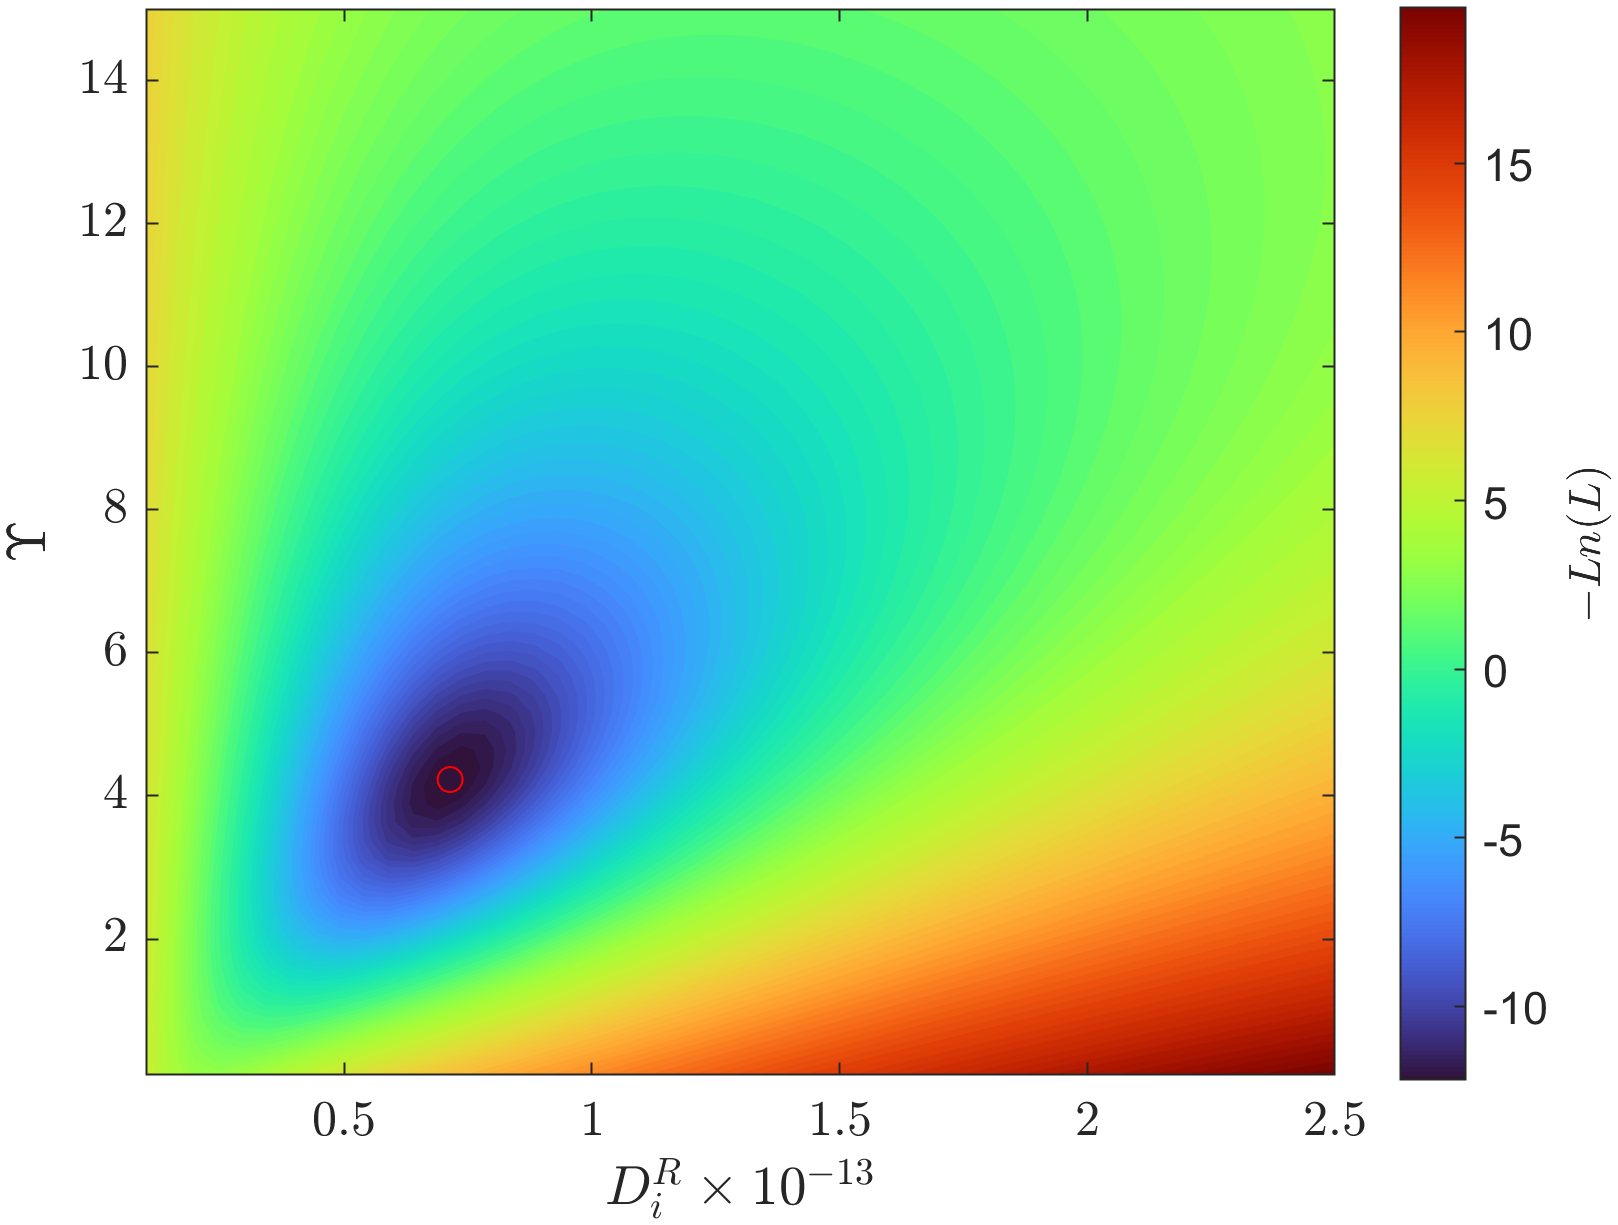
\includegraphics[trim = 0.0cm 0.0cm 0.0cm 0.0cm,clip, width=\columnwidth]{/Results_estimation/Parameter_space_Di_Gamma_dataset_1_org.png}
			\caption{The modified model}
			\label{fig: Fit_1_Di_Gamma}
		\end{subfigure}
		\caption{Parameter space for experiment 1}
		%\label{fig: Fit_Di_Gamma}
	\end{figure}
		
	{\footnotesize
		\begin{equation*}
			\begin{split}
				&\lim_{k_m \rightarrow \infty} \left({\color{black}{\color{black} c_s} }(t,z)  - \cfrac{{\color{black}\rho_s}}{{\color{black}k_m}(T(t,z)){\color{black}\rho}(T(t,z),{\color{black}P}(t))}  c_f \right)  = \\
				&= \left({\color{black}{\color{black} c_s} }(t,z)  - \cfrac{\rho_s}{\infty \cdot \rho(T(t,z),P(t))}  {c_f}(t,z) \right) = \left(c_s(t,z) - 0 \right)
			\end{split}
	\end{equation*} }
	
	The extraction model can be adapted to incorporate adjustments for the reduced kinetic term and axial diffusion. In this revised setup, two parameters remain undetermined: the internal diffusion coefficient $D_i$ and the axial diffusion coefficient $D_e^M$. Figure \ref{fig: Fit_1_Di_Dx} illustrates the parameter space of the modified model and associated cost function values.
		
	Similarly to the previous case, the optimal value of $D_i$ exists, but a unique value for the $D_e^M$ cannot be determined. Figure \ref{fig: Fit_1_Di_Dx} illustrates the minimal impact of the axial diffusion coefficient, where a broad range of $D_e^M$ yields identical cost function values. By selecting a low value $D_e^M$, the axial diffusion terms can be reduced or eliminated from the model without compromising its generality. This observation aligns with the findings of \citet{Rahimi2011}, who analysed the same dataset and reported Peclet numbers ranging between 290 and 400. Such high values of the Peclet number suggest that the advection term dominates the mass transfer, and the axial diffusion is negligible.
	
	In both scenarios previously discussed, the fitting outcomes were not deemed satisfactory. Building upon the concepts underlying the Broken-and-Intact and Shrinking Core models (detailed in Chapter \ref{CH: Gamma_Function}), the $\gamma$-function is introduced to capture the decreasing extraction kinetics. The correction factor is combined with the simplified linear model, resulting in a two-parameter model ($D_i^R$ and $\Upsilon$) as given by Equation \ref{Model_kinetic}. Figure \ref{fig: Fit_1_Di_Gamma} shows the parameter space and the corresponding cost function values.
		
	\begin{figure}[!h]
		\centering
		\begin{subfigure}{0.66\columnwidth}
			\centering
			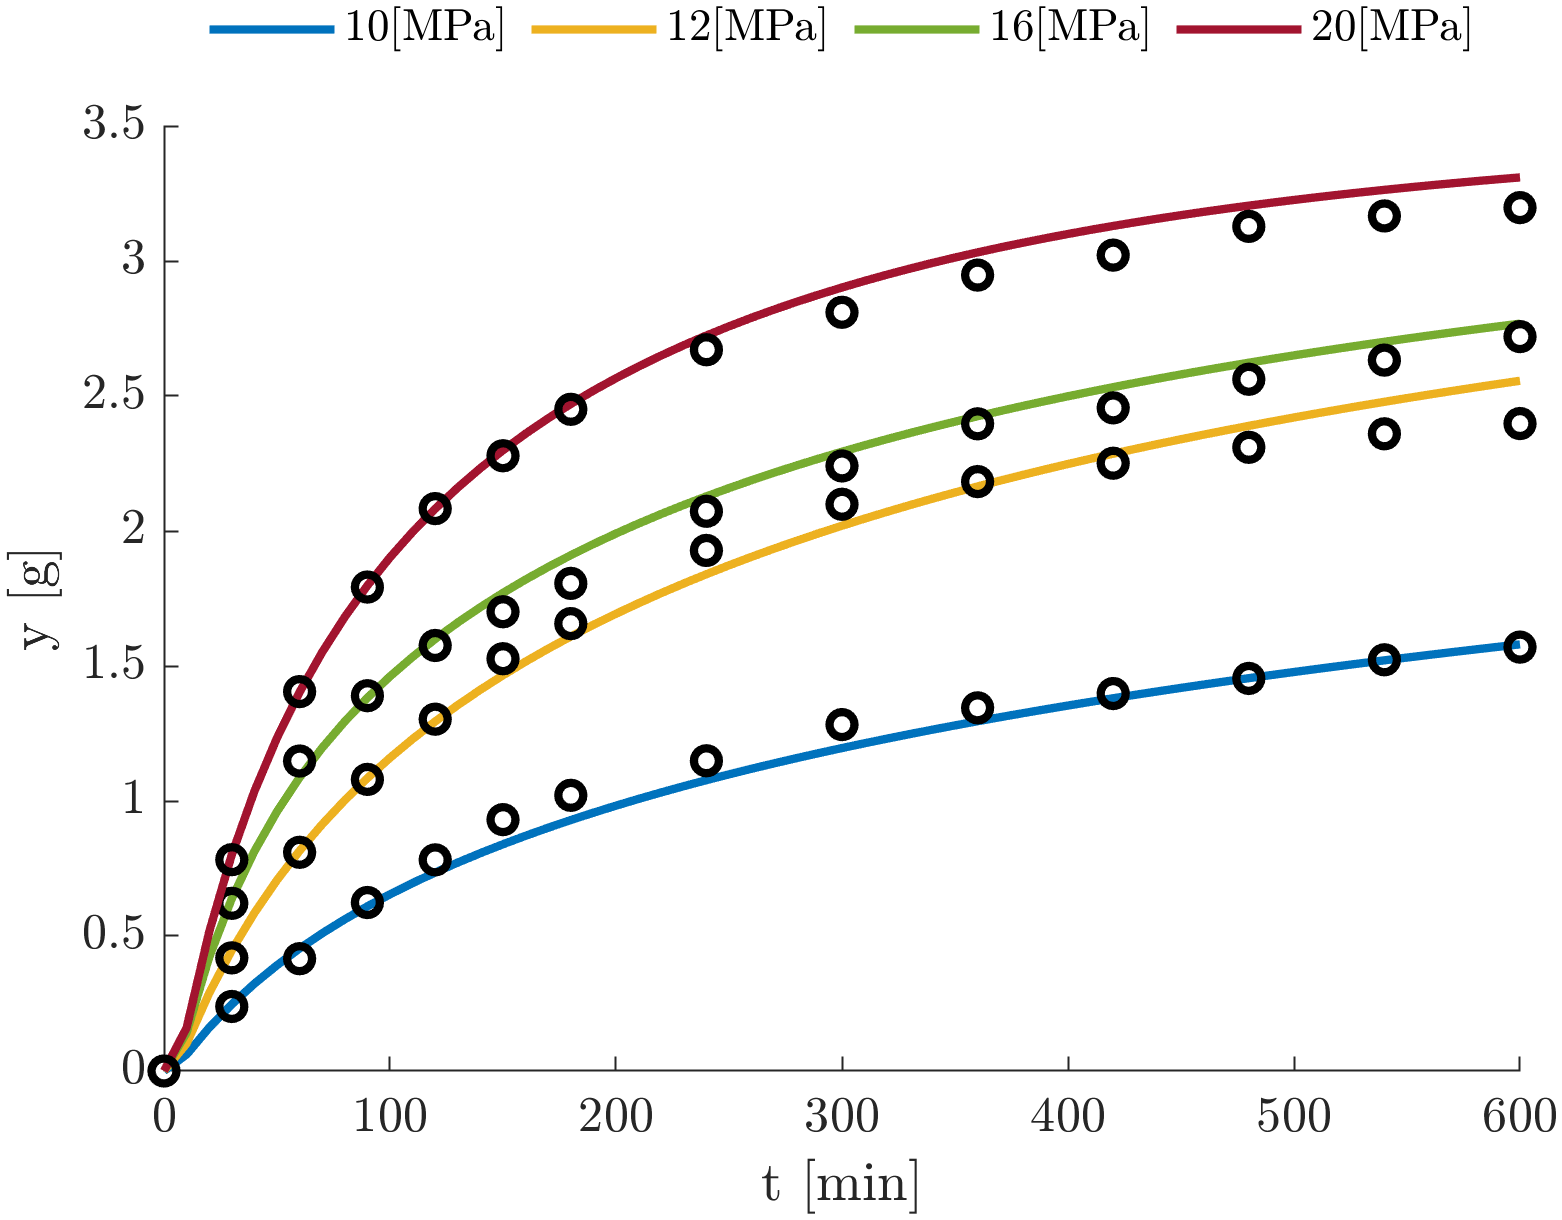
\includegraphics[trim = 0.0cm 0.0cm 0.0cm 0.0cm,clip, width=\columnwidth]{/Results_estimation/Fit_Di_Gamma_1_4.png}
			\caption{Parameter estimation results at $6.67\times 10^{-5}$ [kg/s] and temperature of 40 $[^\circ C]$}
			\label{fig: Fit_1_4_Di_Gamma}
		\end{subfigure}
		\hfill
		\begin{subfigure}{0.66\columnwidth}
			\centering
			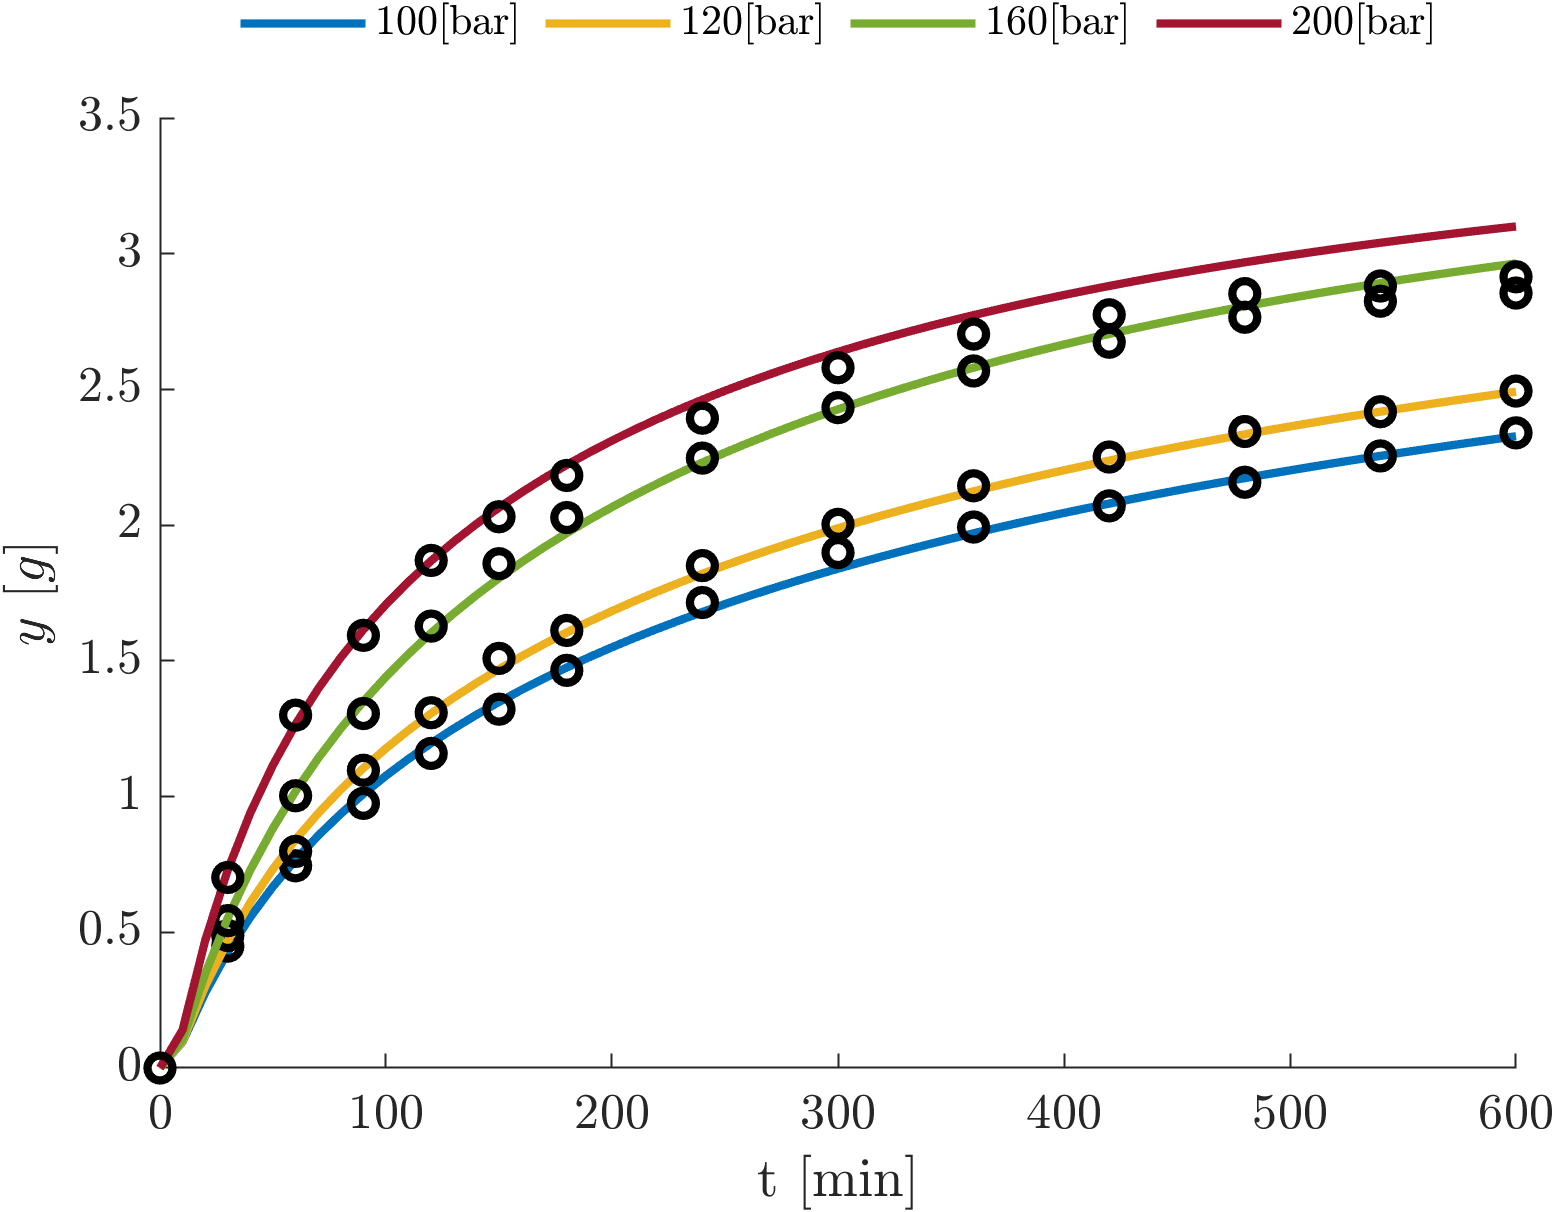
\includegraphics[trim = 0.0cm 0.0cm 0.0cm 0.0cm,clip, width=\columnwidth]{/Results_estimation/Fit_Di_Gamma_5_8.png}
			\caption{Parameter estimation results at $6.67\times 10^{-5}$ [kg/s] and temperature of 30 $[^\circ C]$}
			\label{fig: Fit_5_8_Di_Gamma}
		\end{subfigure}
		\hfill
		\begin{subfigure}{0.66\columnwidth}
			\centering
			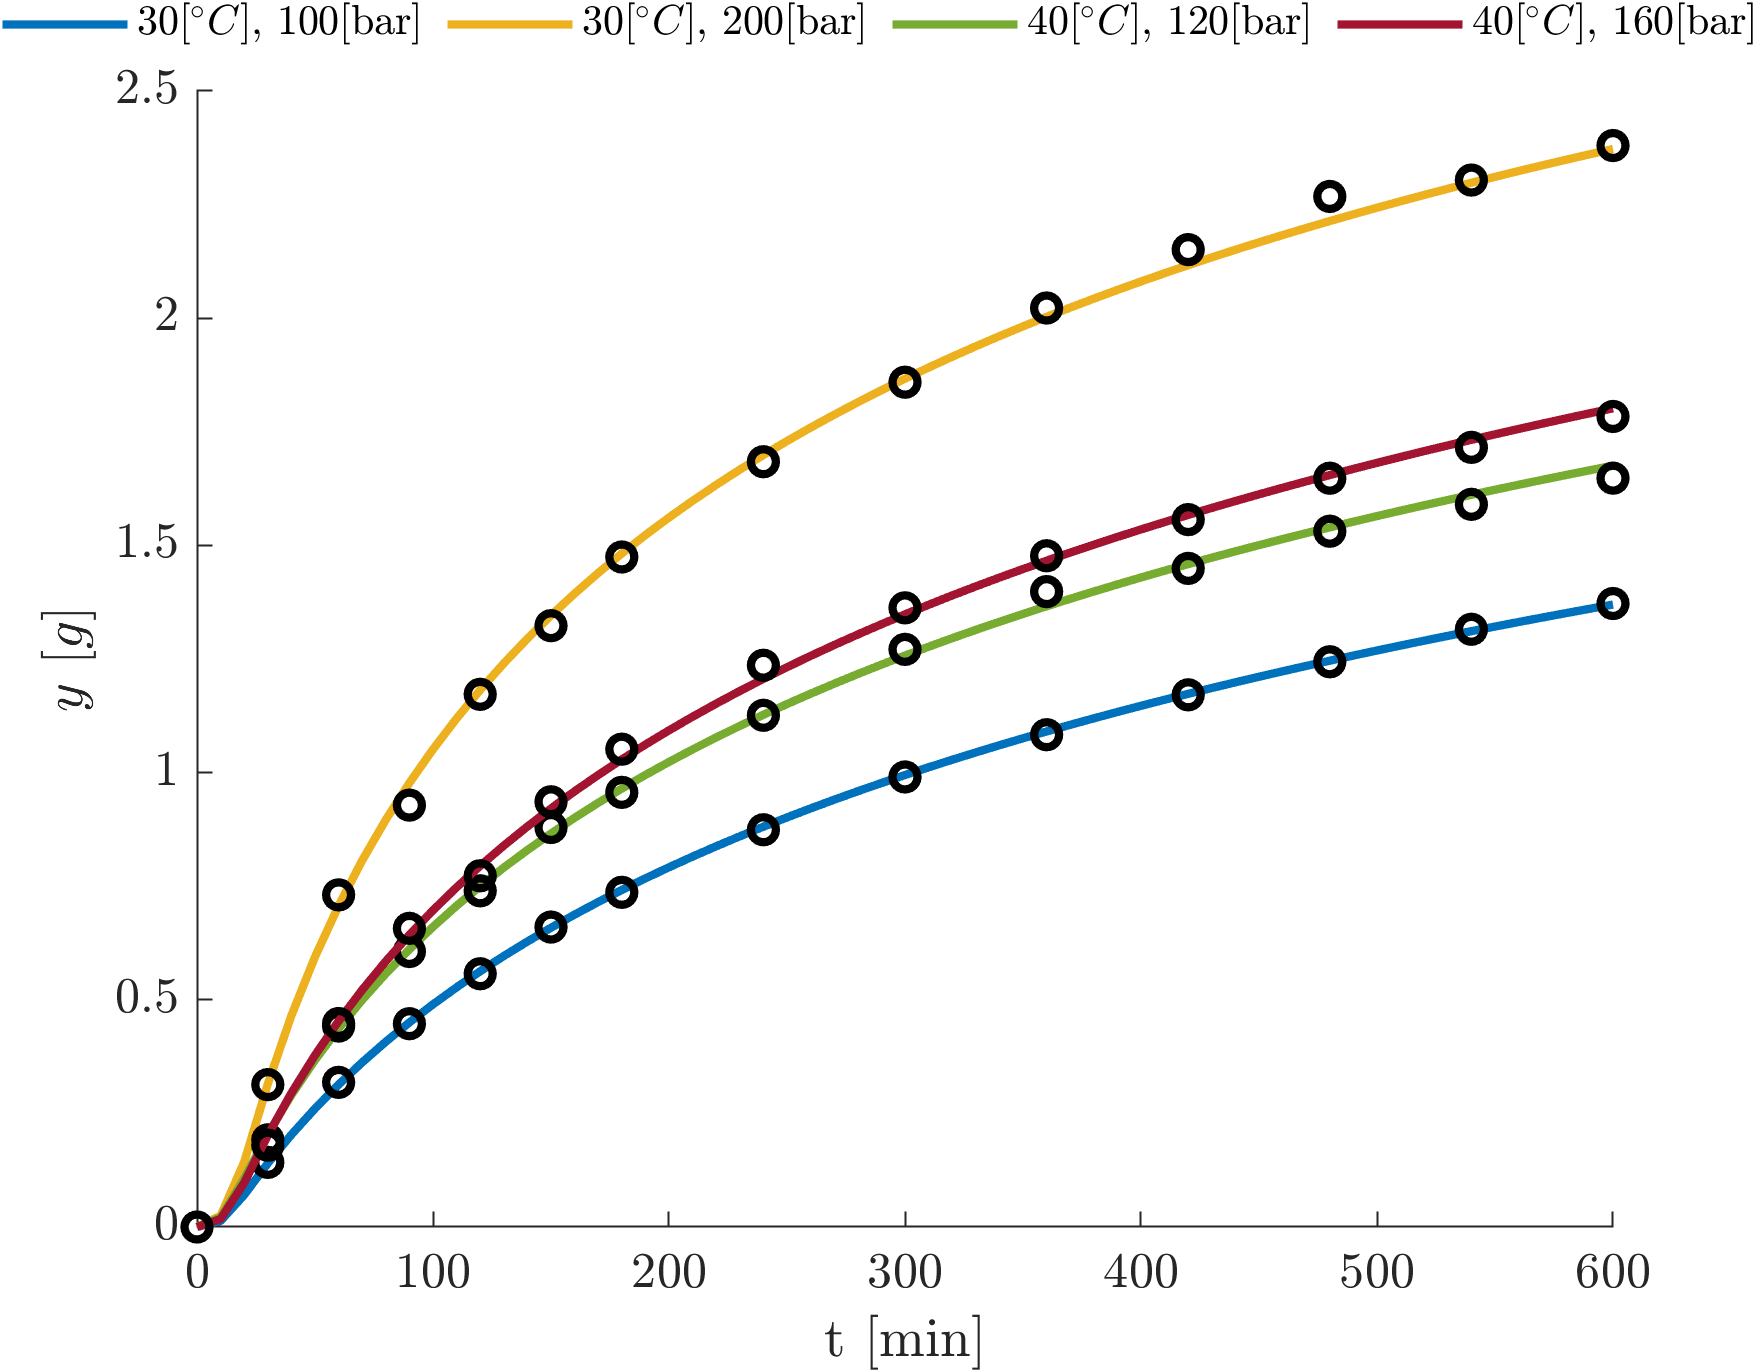
\includegraphics[trim = 0.0cm 0.0cm 0.0cm 0.0cm,clip, width=\columnwidth]{/Results_estimation/Fit_Di_Gamma_9_12.png}
			\caption{Results of parameter estimation for experiments at $3.33\times 10^{-5}$ [kg/s]}
			\label{fig: Fit_9_12_Di_Gamma}
		\end{subfigure}
		\caption{Parameter estimation results obtained from the modified model}
		\label{fig: Fit_Di_Gamma}
	\end{figure}
	
	The parameter space for the modified model exhibits a distinct minimum value corresponding to the solution of the parameter estimation problem for experiment 1. The red circle highlights the minimum value of the cost function found by the optimizer. The remaining experiments are fitted to the modified extraction model, and results, presented in Figure \ref{fig: Fit_Di_Gamma}, show good agreement with experimental data. 
			
	\iffalse
	The estimated parameters describe the diminishing trend of the internal diffusion coefficient $D_i$, as delineated by Equation \ref{EQ: C_sat_function}. It is hypothesized that the internal diffusion coefficient decreases because solute particles face greater difficulty diffusing from the core of a particle than from positions closer to the surface. Decay patterns under various operational conditions, depicted in Figure \ref{fig: Gamma_function}, show that the internal diffusion coefficient is notably higher in fluids under high pressure. This observation aligns with the findings of \citet{Giddings1968}, \citet{Gurdial1989}, and \citet{Machida2011}, who explored the solvation capability of solvents and its correlation with the physical properties of CO$_2$ by calculating the Hildebrand solubility parameter $\delta_H$. \citet{Giddings1968} introduced a correlation for the solubility parameter $\delta_H[\text{MPa}^{1/2}] = 1.25 P_c^{1/2}\rho_r$, with $P_c$ and $\rho_r$ representing the critical pressure and reduced density, respectively. Similarly, \citet{Marcus2006} formulated a correlation based on the Van der Waals equation of state: $\delta_H[\text{MPa}^{1/2}] = 2.79 P_c^{1/4}T_r^{1/4}\rho_r$. As Figure \ref{fig: Gamma_function} shows, fluids with higher solubility factors exhibit greater internal diffusion coefficients. However, the relationship between $\delta_H$ and $D_i$ should be considered indicative rather than definitive due to the non-ideal nature of the system and the omission of external factors such as fluid velocity.
	
	\begin{figure}[!h]
		\centering
		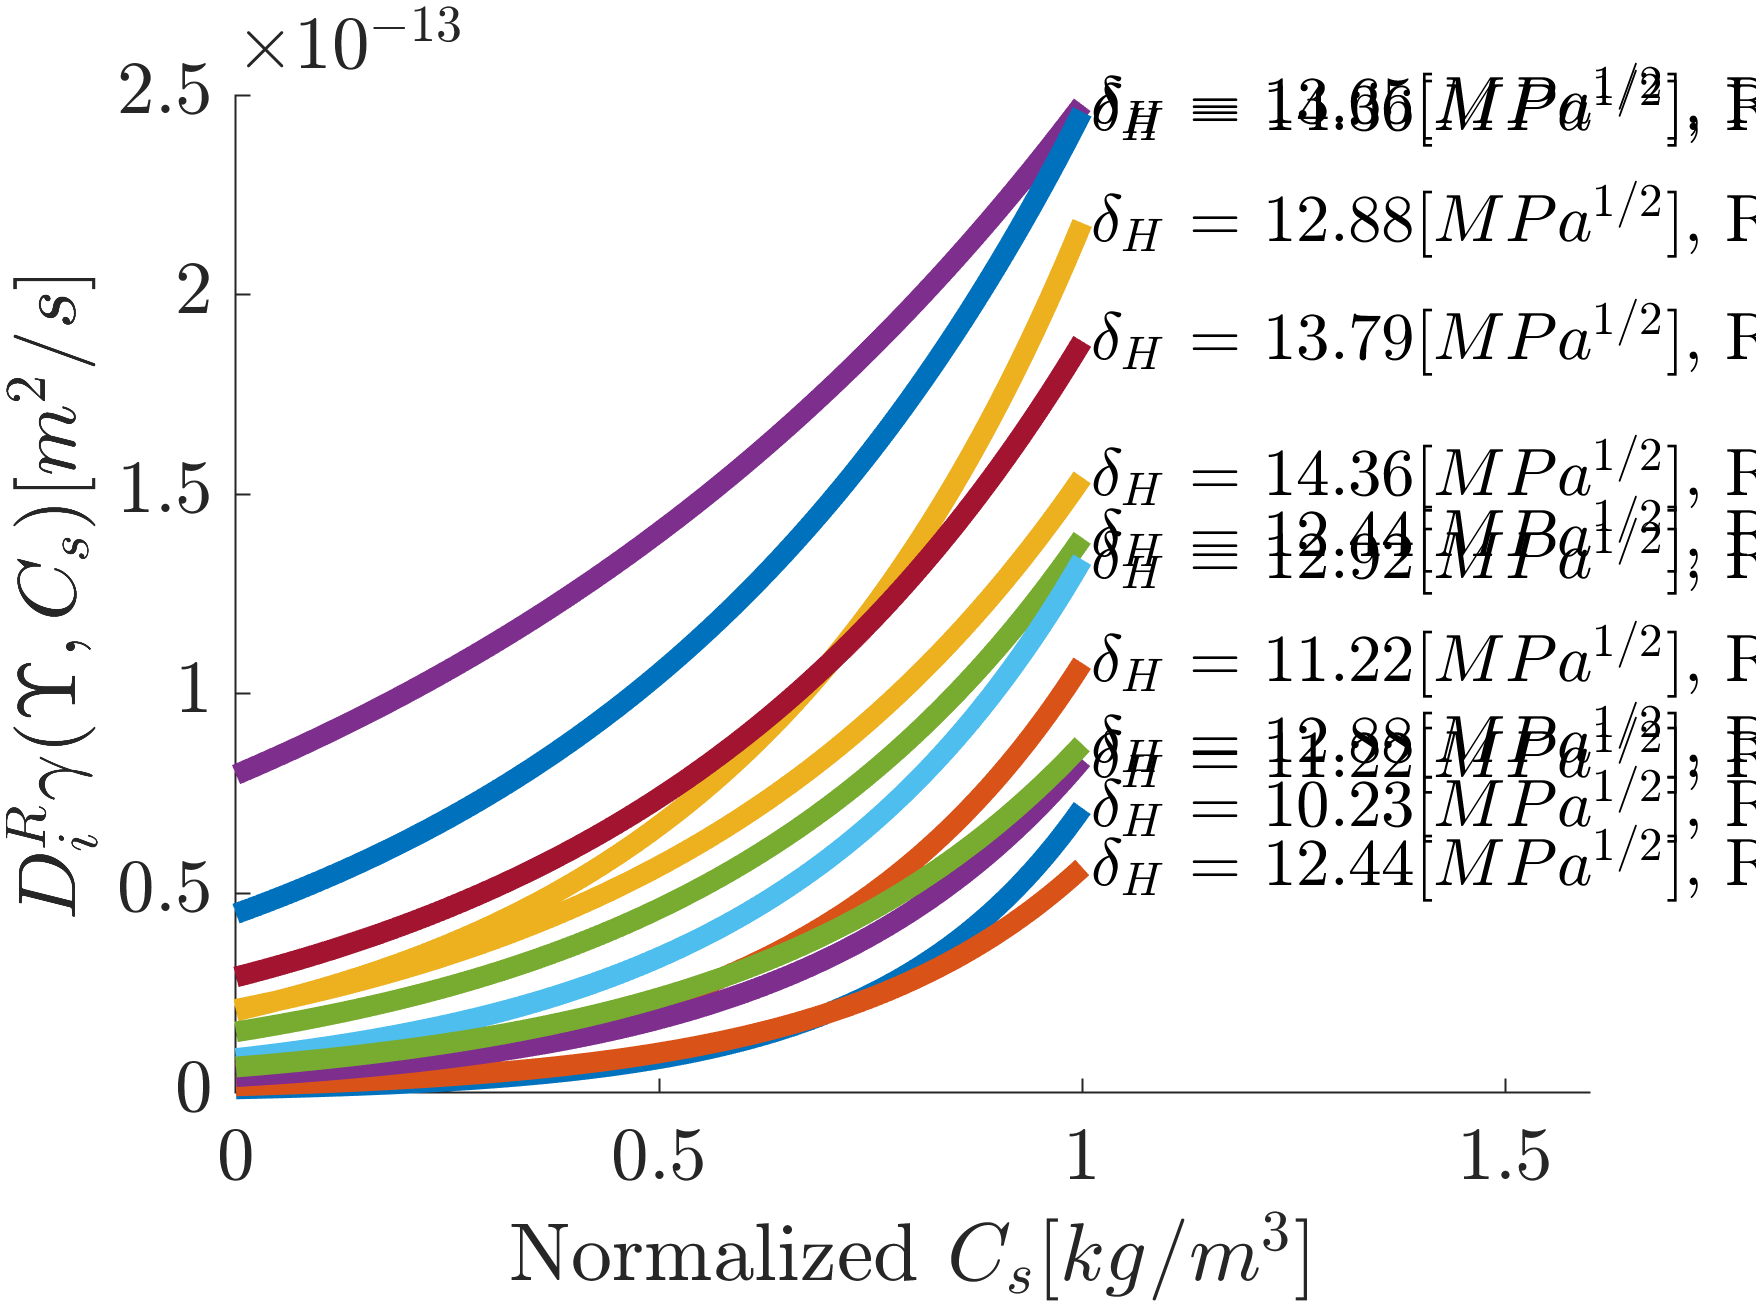
\includegraphics[trim = 0.0cm 0.0cm 0.0cm 0.0cm,clip, width=\columnwidth]{/Results_estimation/Gamma_function.png}
		\caption{The decaying internal diffusion coefficient}
		\label{fig: Gamma_function}
	\end{figure}
		
	\fi	
		
	The parameter estimation results are combined to analyse the relationship between the obtained parameters and the operating conditions. Unlike traditional methods that employ a combination of Reynolds, Schmidt, and Sherwood numbers to find correlations—omitted here due to the insignificance of axial diffusion—the approach in this study leverages the Reynolds number $\left(Re = \frac{(2r) \cdot \rho_f \cdot u}{\mu}\right)$ as the sole independent variable. Using the Reynolds number has the advantage of considering the influence of all the control variables (temperature, pressure and flow rate), which means it can be uniquely defined by selecting operating conditions.	
	
	\begin{figure}[!h]
		\centering
		\begin{subfigure}{0.48\columnwidth}
			\centering
			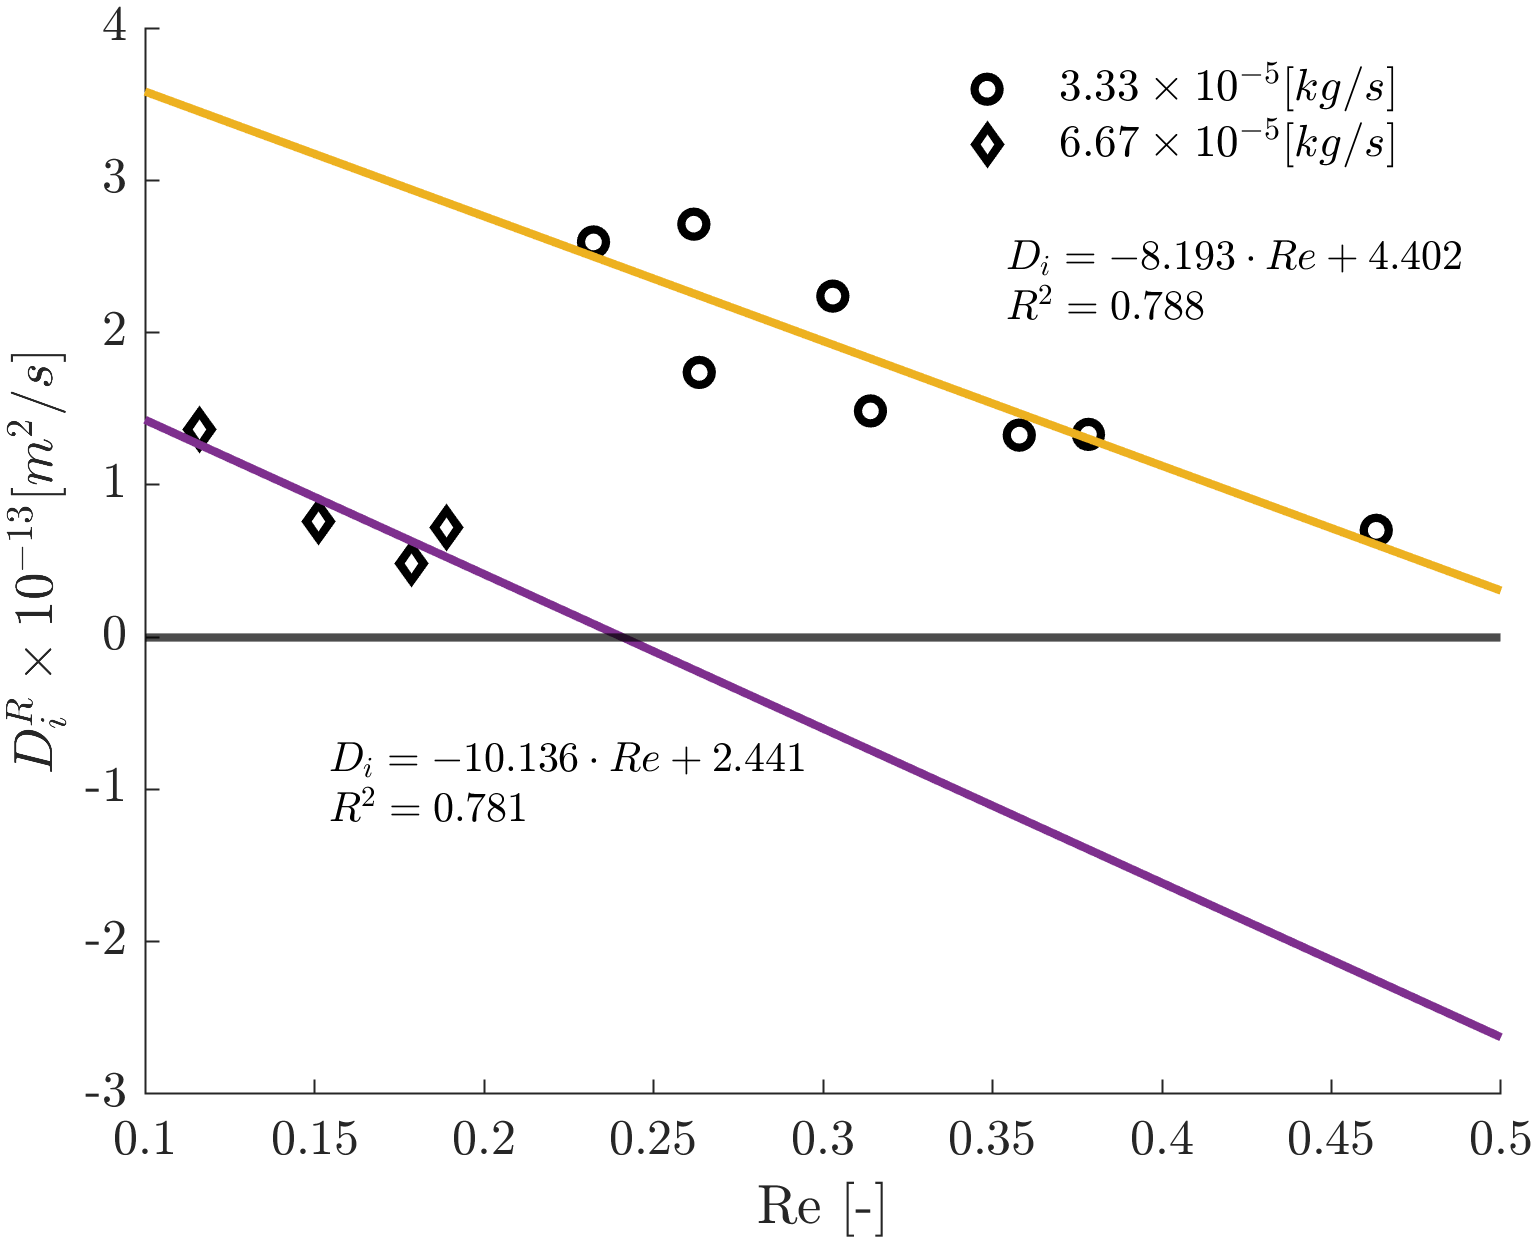
\includegraphics[trim = 0.0cm 0.0cm 0.0cm 0.0cm,clip, width=\columnwidth]{/Results_estimation/Correlation_Di_Re.png}
			\caption{Linear regression $D_i^R = f(Re)$}
			\label{fig: Correlations_Di_Re}
		\end{subfigure}
		\hfill
		\begin{subfigure}{0.48\columnwidth}
			\centering
			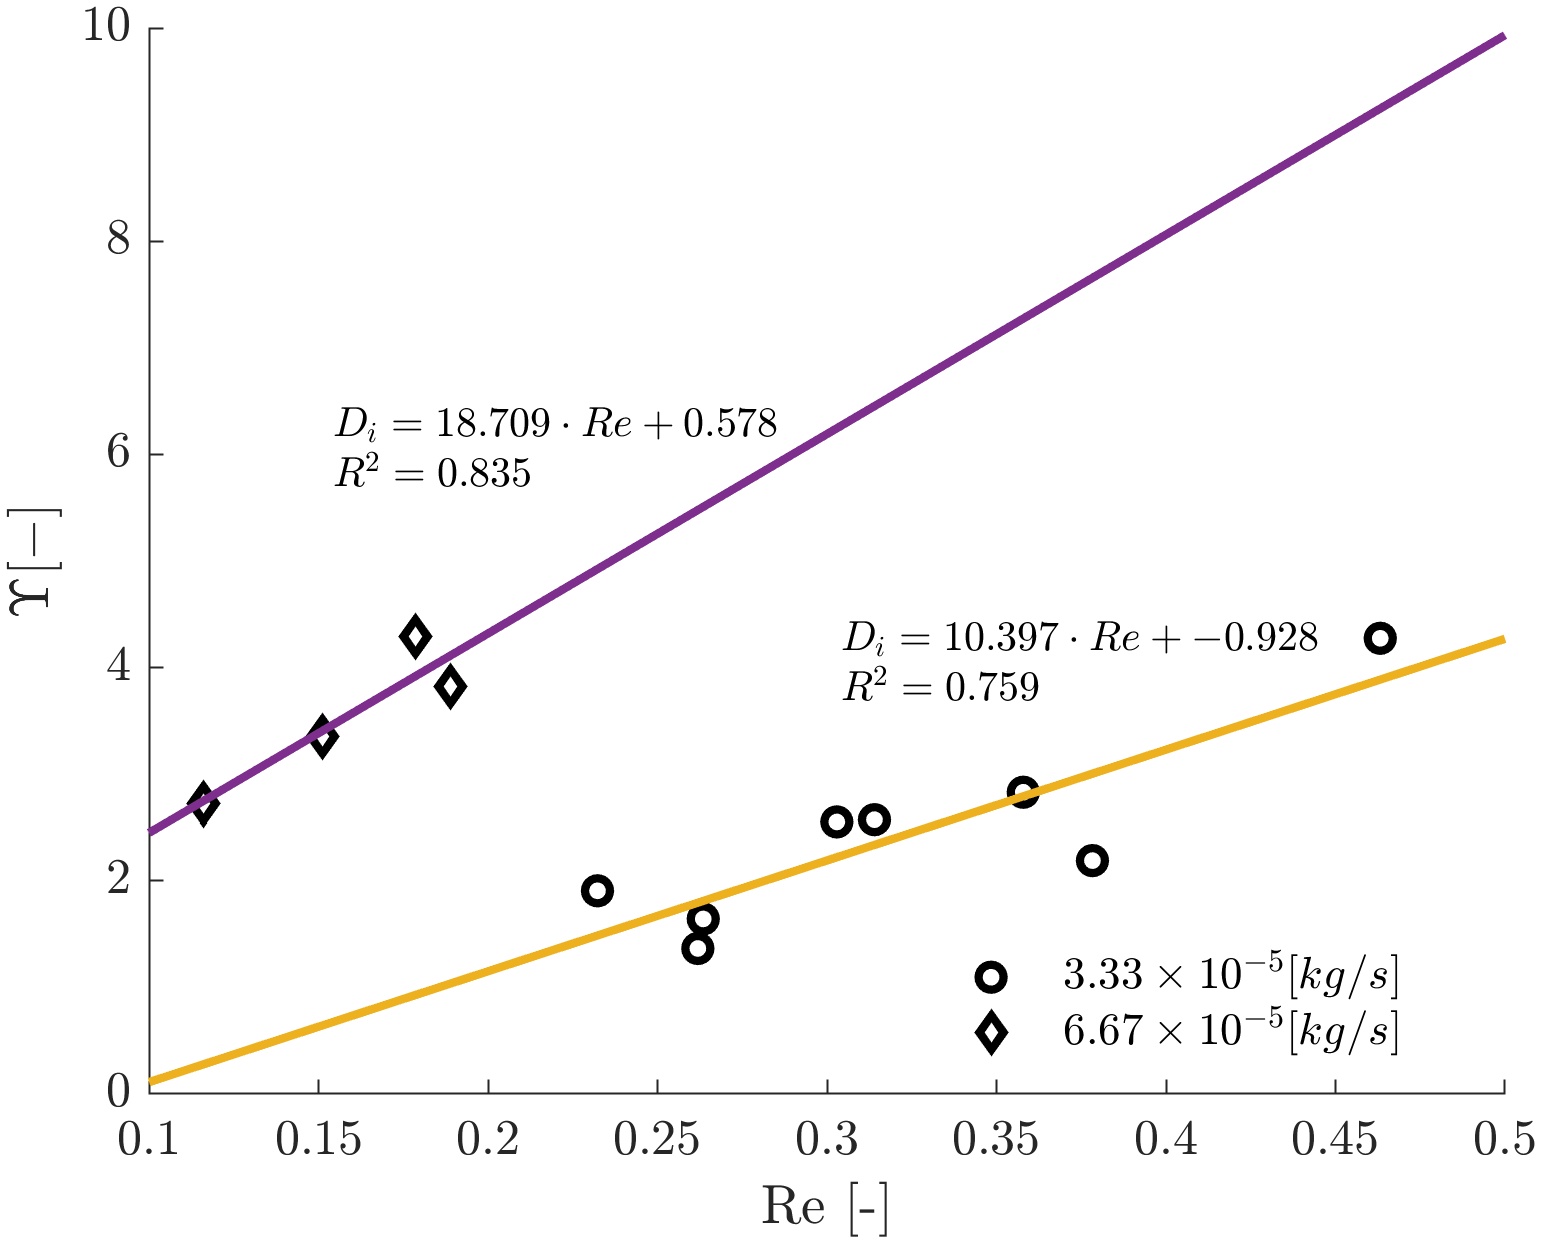
\includegraphics[trim = 0.0cm 0.0cm 0.0cm 0.0cm,clip, width=\columnwidth]{/Results_estimation/Correlation_Gamma_Re.png}
			\caption{Linear regression $\Upsilon = f(Re)$}
			\label{fig: Correlations_Gamma_Re}
		\end{subfigure}
		\hfill
		\begin{subfigure}{0.48\columnwidth}
			\centering
			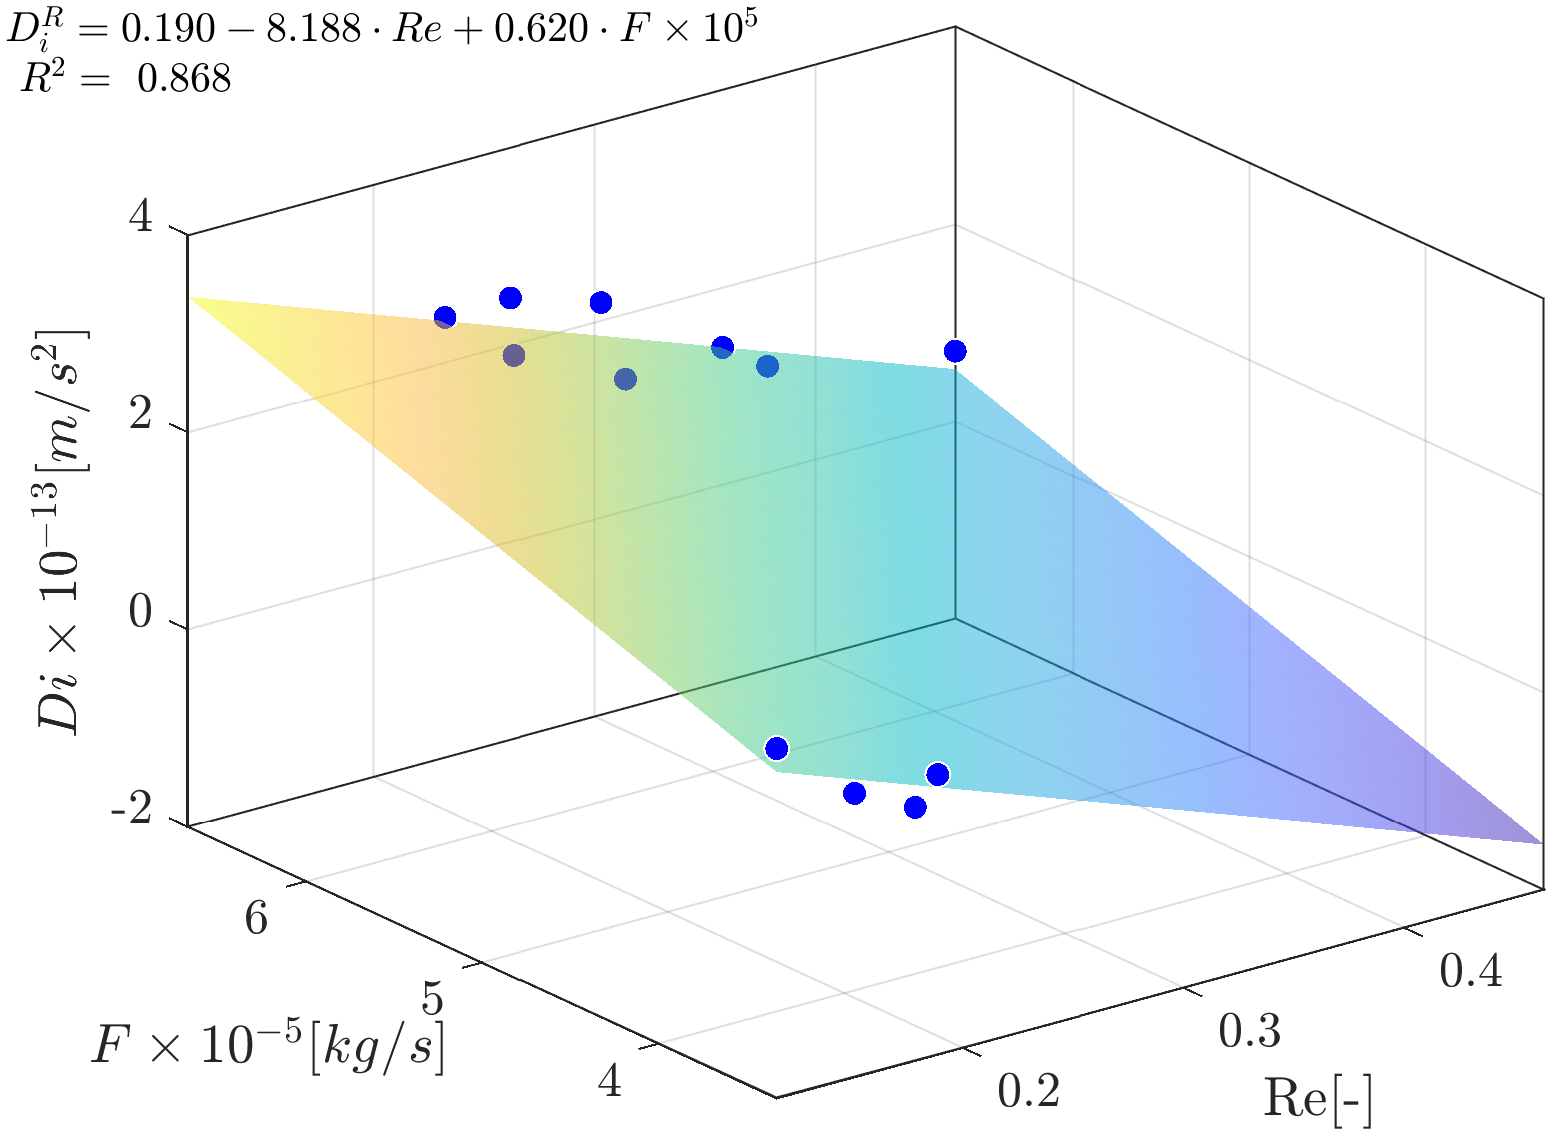
\includegraphics[trim = 0.0cm 0.0cm 0.0cm 0.0cm,clip, width=\columnwidth]{/Results_estimation/Di_Re_F.png}
			\caption{Multiple linear regression $D_i^R = f(Re, F)$}
			\label{fig: Correlations_Di_Re_F}
		\end{subfigure}
		\hfill
		\begin{subfigure}{0.48\columnwidth}
			\centering
			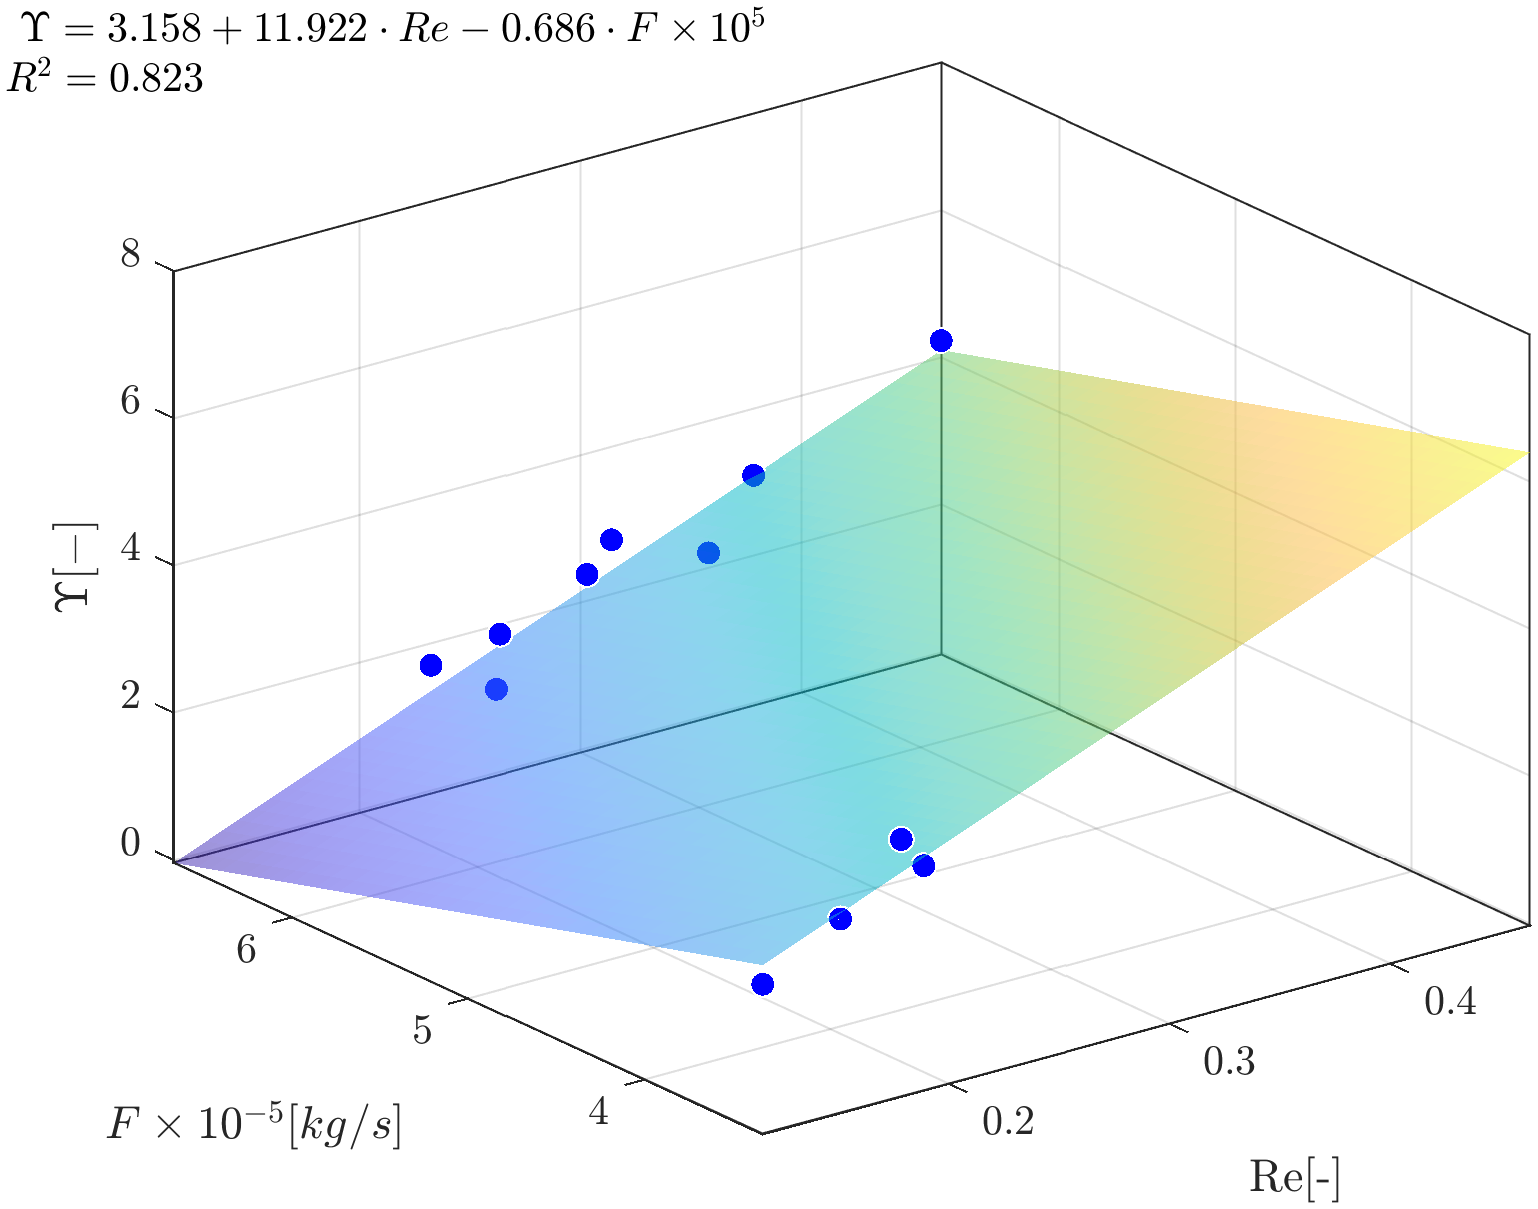
\includegraphics[trim = 0.0cm 0.0cm 0.0cm 0.0cm,clip, width=\columnwidth]{/Results_estimation/Gamma_Re_F.png}
			\caption{Multiple linear regression $\Upsilon = f(Re, F)$}
			\label{fig: Correlations_Gamma_Re_F}
		\end{subfigure}
		\caption{Empirical correlations between parameters}
		%\label{fig: Correlations_surface}
	\end{figure}
	
	
	In Figures \ref{fig: Correlations_Di_Re} and \ref{fig: Correlations_Gamma_Re}, two distinct data clusters emerge, each corresponding to a different mass flow rate. Despite the linear trends observed in both sets of correlations, the correlations for $D_i^R$ exhibit a decline with increasing Re, whereas those for $\Upsilon$ show an upward trend with Re. The decrease in $D_i^R$ across each data line can be attributed to higher fluid density and increased mass transfer resistance. %Conversely, the rise in $\Upsilon$ correlations may be explained by enhanced solubility. The Hildebrand solubility factor and the Reynolds number are proportional to the fluid density; hence, $\Upsilon$ can be correlated with Re.
	
	A more general relationship can be obtained by applying multiple linear regression instead of linear regression. The clusters in Figure \ref{fig: Correlations_Di_Re}  and \ref{fig: Correlations_Gamma_Re} are close to parallel, suggesting that a plane would combine all the data points. The Reynolds number and flow rate act as independent variables for $D_i^R$ and $\Upsilon$ as presented in Figures \ref{fig: Correlations_Di_Re_F} and \ref{fig: Correlations_Gamma_Re_F}. The presented correlations are valid in the whole range of investigated operating conditions.
	
	\begin{figure}[!h]
		\centering
		\begin{subfigure}{0.66\columnwidth}
			\centering
			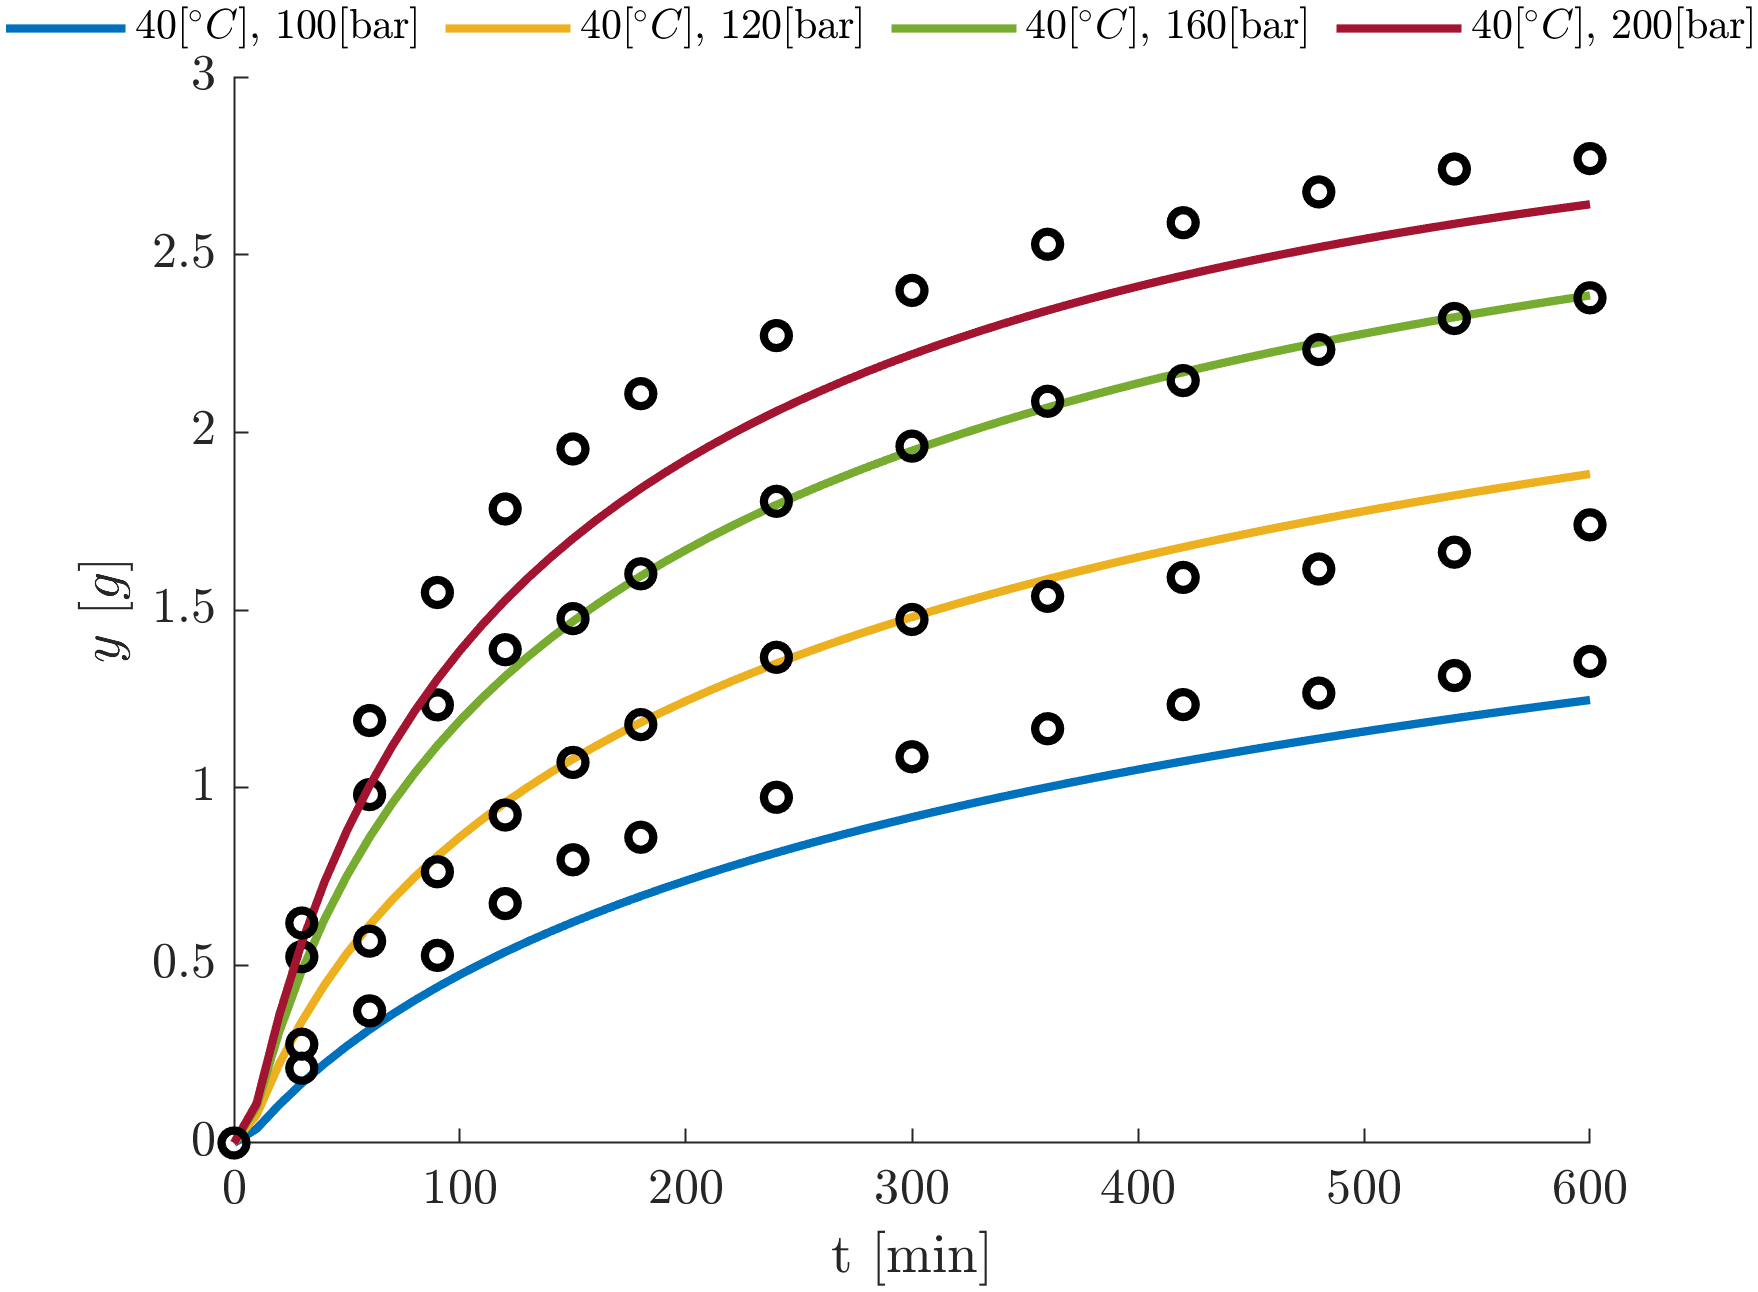
\includegraphics[trim = 0.0cm 0.0cm 0.0cm 0.0cm,clip, width=\columnwidth]{/Results_estimation/Fit_Di_Gamma_1_4_correlation.png}
			\caption{Simulation results obtained at $6.67\times 10^{-5}$ [kg/s] and temperature of 40 $[^\circ C]$}
			\label{fig: Fit_1_4_Di_Gamma_correlation}
		\end{subfigure}
		\hfill
		\begin{subfigure}{0.66\columnwidth}
			\centering
			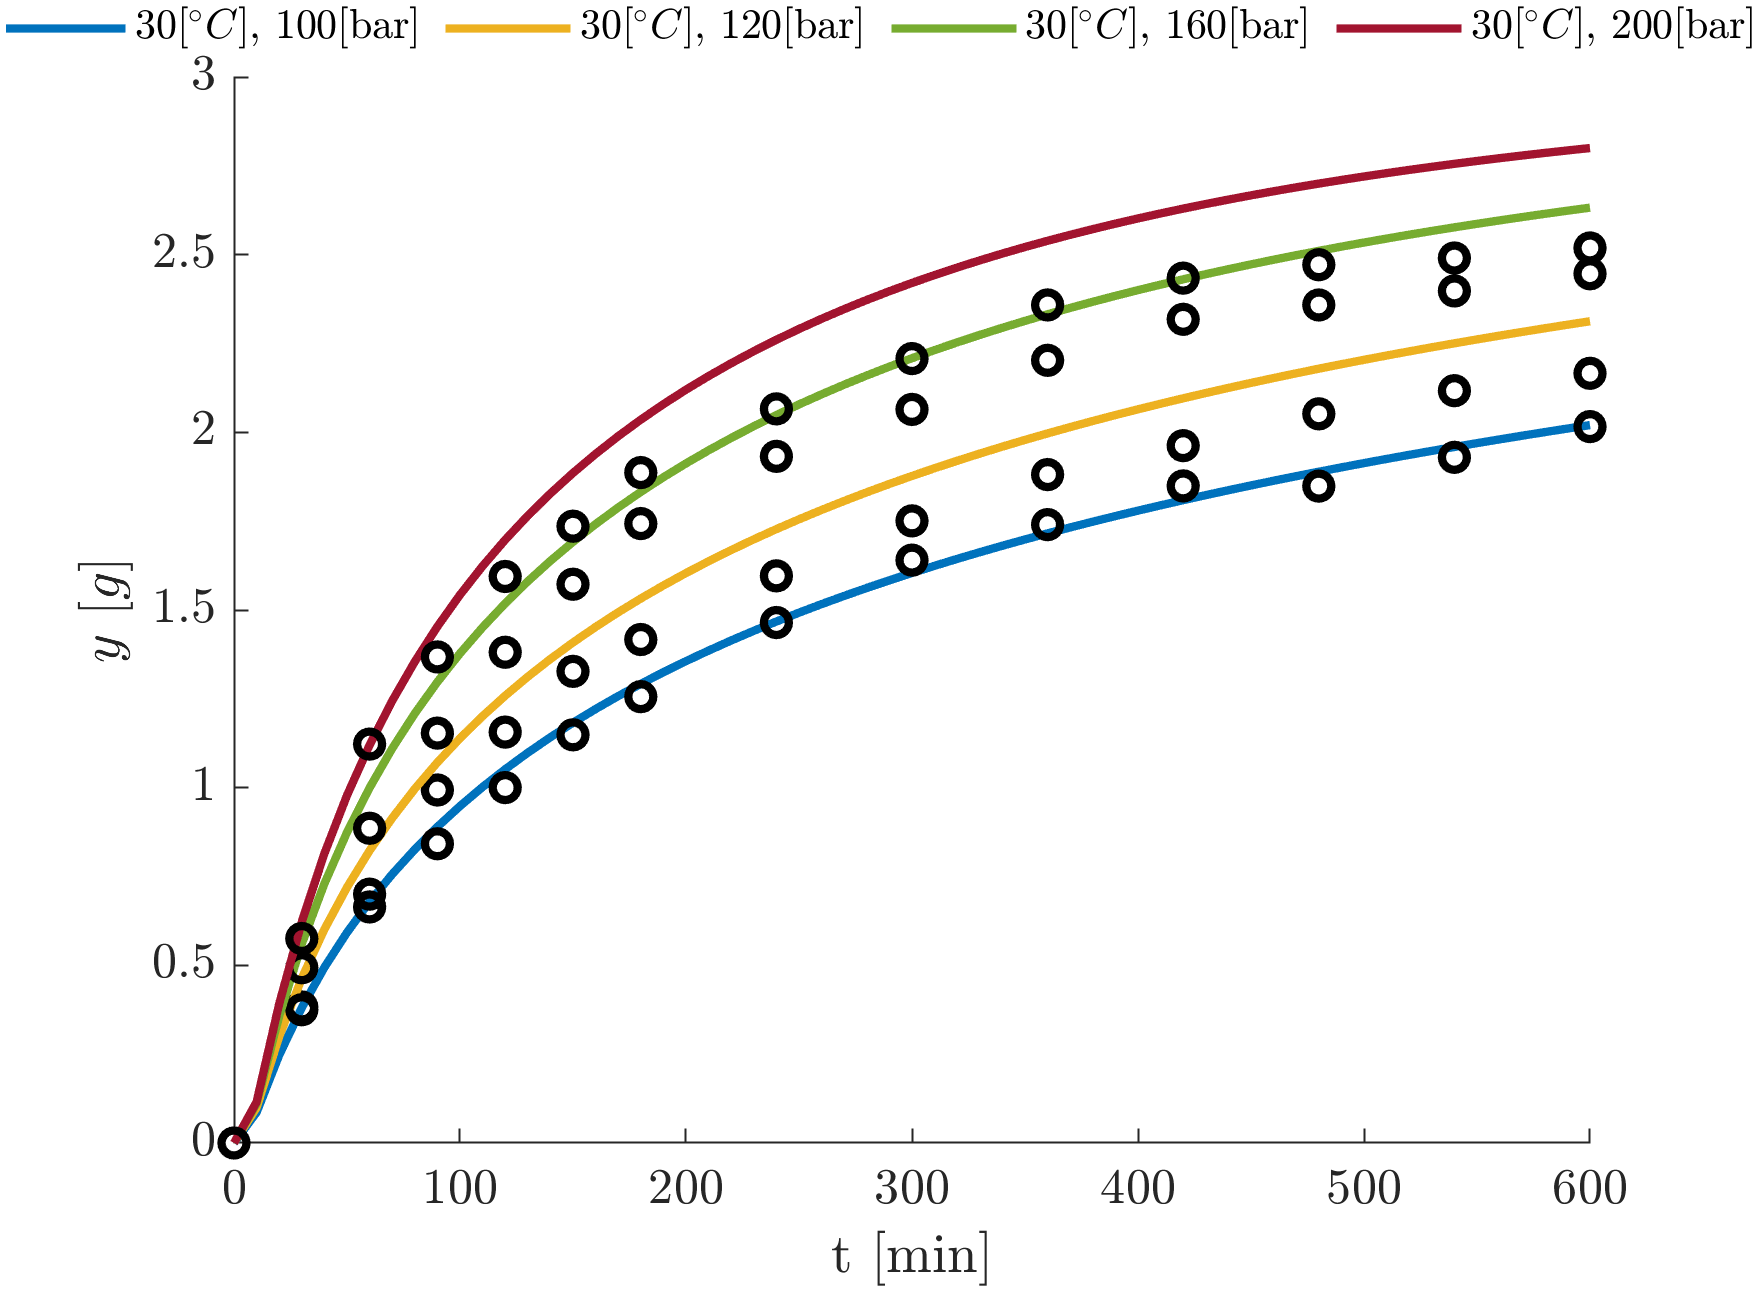
\includegraphics[trim = 0.0cm 0.0cm 0.0cm 0.0cm,clip, width=\columnwidth]{/Results_estimation/Fit_Di_Gamma_5_8_correlation.png}
			\caption{Simulation results obtained at $6.67\times 10^{-5}$ [kg/s] and temperature of 30 $[^\circ C]$}
			\label{fig: Fit_5_8_Di_Gamma_correlation}
		\end{subfigure}
		\hfill
		\begin{subfigure}{0.66\columnwidth}
			\centering
			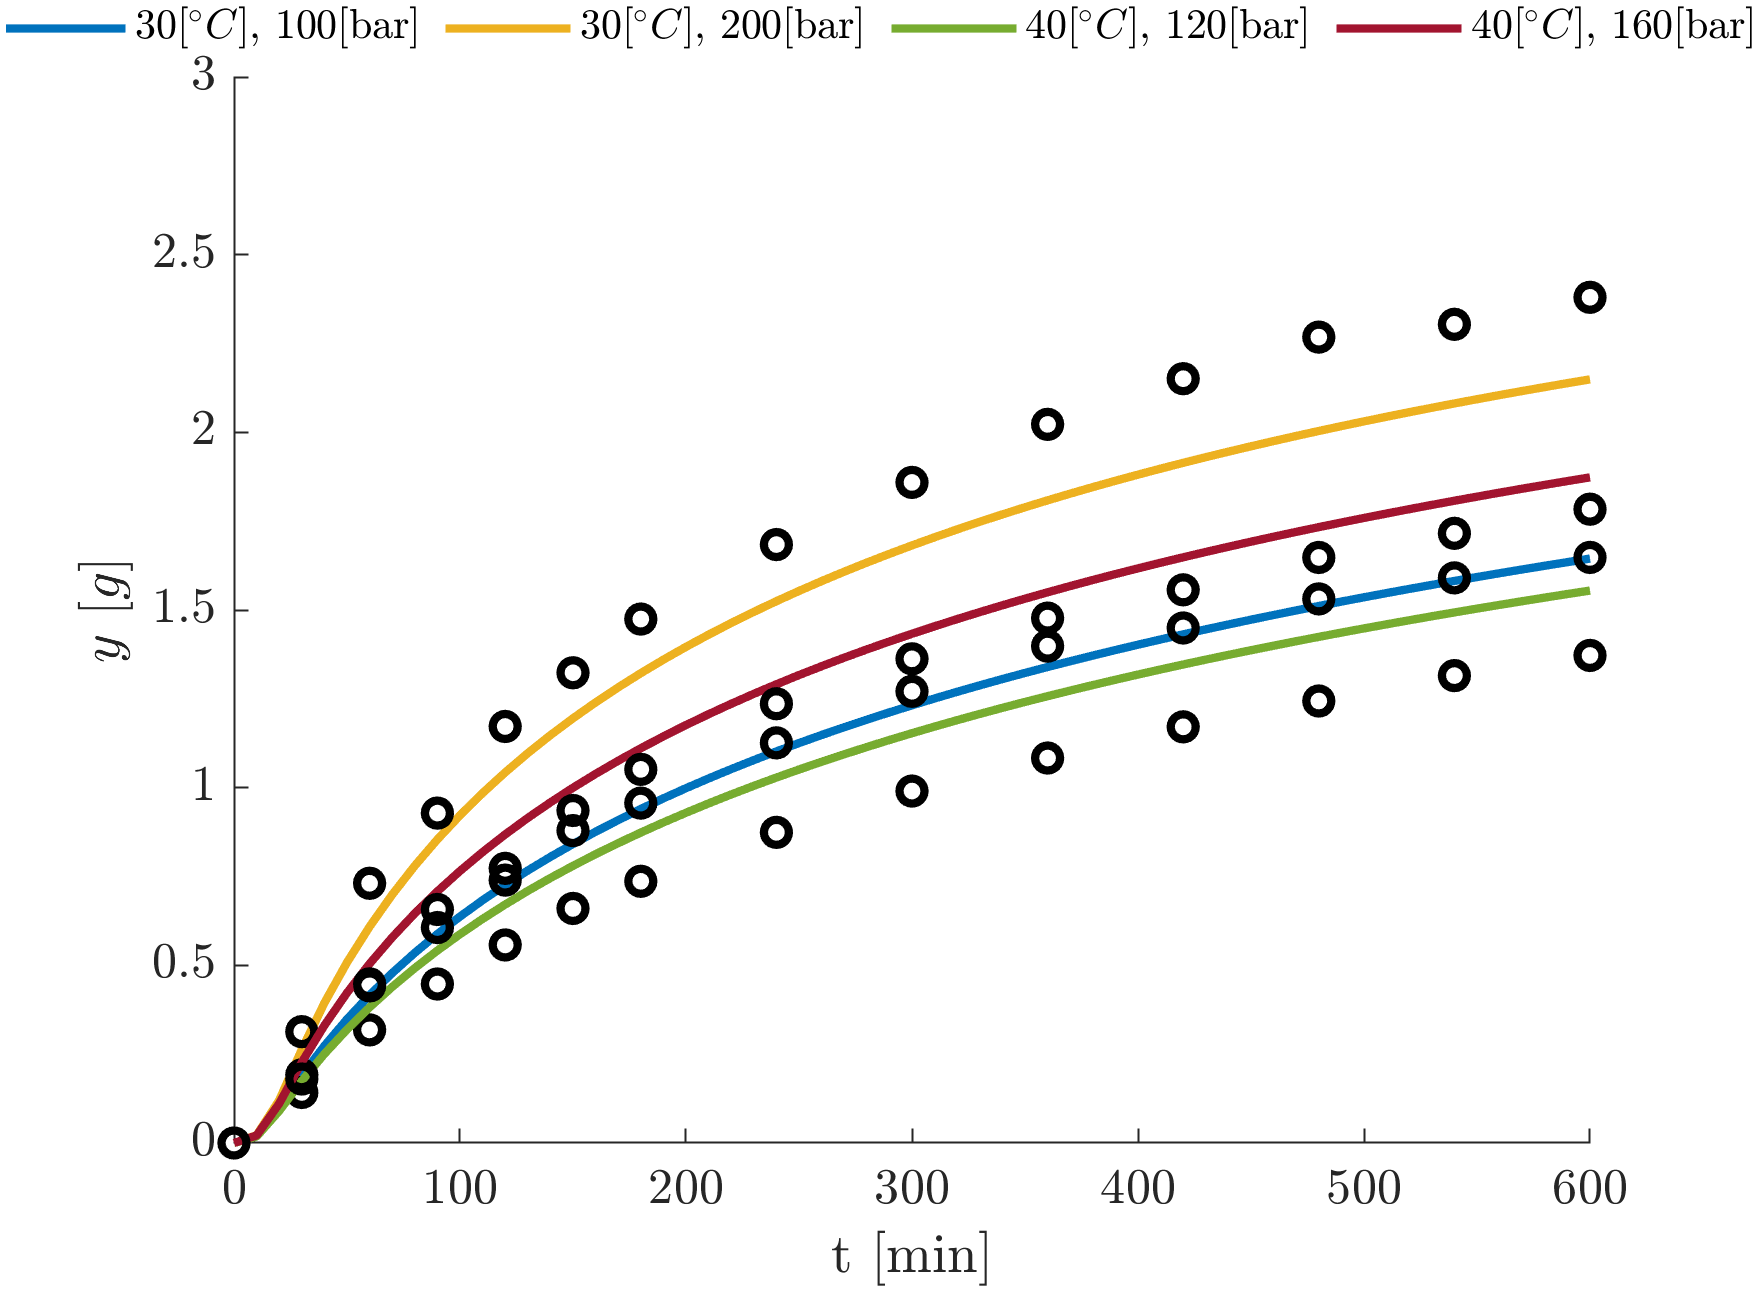
\includegraphics[trim = 0.0cm 0.0cm 0.0cm 0.0cm,clip, width=\columnwidth]{/Results_estimation/Fit_Di_Gamma_9_12_correlation.png}
			\caption{Simulation results obtained at $3.33\times 10^{-5}$ [kg/s]}
			\label{fig: Fit_9_12_Di_Gamma_correlation}
		\end{subfigure}
		\caption{Simulation results from the modified model and correlations}
		\label{fig: Fit_Di_Gamma_correlation}
	\end{figure}
	
	The correlations are later used against the original dataset to show that the correlations can reproduce the results with satisfactory accuracy. Figure \ref{fig: Fit_Di_Gamma_correlation} shows the results of the simulations with incorporated correlations. A good agreement between simulation results and the dataset can be observed. If Figures \ref{fig: Fit_Di_Gamma} and \ref{fig: Fit_Di_Gamma_correlation} are compared, a decrease in the accuracy of simulations can be observed. Such a behaviour is expected due the bias–variance trade-off, which describes the relationship between a model's complexity and the accuracy of its predictions.
	
	%The parameter estimation results are compared to the work of \citet{Povh2001}, who fitted the Sovova model to the same dataset. It should be noted that the \citet{Povh2001} use as the initial solute mass ratio a value of 10\% above the total amount of extract for every experimental, while in this work, the initial conditions are the same for all the experiments as explained above. Contrary to this work, \citet{Povh2001} has not used any numerical solver in his work but rather a combination of analytical methods and a trial and error procedure. \citet{Povh2001} stated that 'the direct fitting of experimental data to the Sovova's model produced parameters that could not be accepted after a careful physical interpretation of the system'. The parameters found in this work seem to have a physical interpretation, and their values are in the excerpted range. 
	
	%\citet{Rahimi2011} fitted the same dataset to a model with desorption–dissolution–diffusion mechanism. To decrease the number of parameters to be found, \citet{Rahimi2011} applied a set of correlations. The remaining parameters were found using a genetic algorithm to solve the parameter estimation problem for each experiment separately. The results obtained by \citet{Rahimi2011} show that the desorption–dissolution–diffusion model cannot reproduce the yield data. The desorption–dissolution–diffusion model and the model used in this work are structurally similar, with the main difference of $\gamma$ function. The $\gamma$ function increases the model's flexibility and allows it to obtain a better fit.
	
	%For every single experiment, \citet{Povh2001} and \citet{Rahimi2011} delivered a set of independent parameters. This work combines the parameters obtained from each experiment to get a single correlation valid for the whole range of investigated operating conditions.
	
	The parameter estimation results are compared against those presented by \citet{Povh2001}, who applied the Sovova model to the same dataset. It is important to note that \citet{Povh2001} use as the initial solute mass ratio a value of 10\% above the total amount of extract for every experimental, while in this work, the initial conditions are the same for all the experiments. In contrast to this work, \citet{Povh2001} did not utilize numerical solvers but used a mix of analytical methodologies and trial-and-error procedures. \citet{Povh2001} remarked that 'the direct fitting of experimental data to the Sovova's model produced parameters that could not be accepted after a careful physical interpretation of the system'. The parameters identified in this study seem to have a physical interpretation and are within the expected range.
	
	\citet{Rahimi2011} analysed the same dataset using the desorption–dissolution–diffusion model. To decrease the number of unknown parameters, \citet{Rahimi2011} applied a set of empirical correlations. The remaining parameters were determined through the use of a genetic algorithm to solve the parameter estimation problem for each experiment individually. Results obtained by \citet{Rahimi2011} shows that the desorption–dissolution–diffusion model fails to reproduce the yield data. The main difference between the model employed by \citet{Rahimi2011} and the one in this study is the $\gamma$-function. The $\gamma$-function increases the model's flexibility by adjusting $D_i$ and allows it to obtain a better fit.
	
	\citet{Povh2001} and \citet{Rahimi2011} delivered a set of independent parameters for every single experiment. This work combines the parameters obtained from each experiment to get a single correlation valid for the whole range of investigated operating conditions.
	
\end{document}













































